\documentclass{beamer}
\usepackage{graphicx}
\usepackage{listings} % Syntax highlighing
\usepackage{listings-golang}
\usepackage{fancyvrb} % Inline verbatim
\usepackage{hyperref} % Hyperlinks
\hypersetup{pdfpagemode=FullScreen}
\usepackage{attachfile}
\usepackage{tikz}
\def\checkmark{\tikz\fill[scale=0.4](0,.35) -- (.25,0) -- (1,.7) -- (.25,.15) -- cycle;}

\usetheme{Boadilla}
\title{Malware Features and Models}
\author{UMBC Malware Data Science}
\date{Week 4: 17 February 2020}

\begin{document}

\begin{frame}{Recap}
    Recap:
    \\ ~~ \\
    Last week, we discussed using features and characteristics from the malware \& goodware collection to build a network showing potential relationships between malware samples. These connections could show common methodologies, tooling, or authors. They might also be coincidence. 
\end{frame}

\begin{frame}{Machine Learning \& Malware}
    The remainder of the course will focus on building machine learning models for malware detection. We need a few key items:
    \only<1> {
    \begin{columns}
        \column{0.7\textwidth} {
                \begin{itemize}
                \item Data corpus: Malware \& Goodware  \checkmark
                \item Feature selection
                \item Feature extraction (build the datasets)
                \item Training on most of the data, $\approx$80\%
                \item Testing on the remaining data
                \item Utilizing metrics to measure performance (there's more than just accuracy)
            \end{itemize}
            }
        \column{0.3\textwidth} {
            ~~
            }
        \end{columns}
    }
    \only<2> {
    \begin{columns}
        \column{0.7\textwidth} {
                \begin{itemize}
                \item Data corpus: Malware \& Goodware  \checkmark
                \item Feature selection
                \item Feature extraction (build the datasets)
                \item Training on most of the data, $\approx$80\%
                \item Testing on the remaining data
                \item Utilizing metrics to measure performance (there's more than just accuracy)
            \end{itemize}
            }
        \column{0.3\textwidth} {
            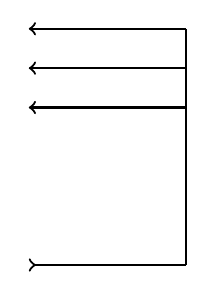
\begin{tikzpicture}
                \draw [>-, thick] (0,1) -- (2,1); % Metrics
                \draw [thick] (2,1) -- (2,4);
                \draw [->, thick] (2,4) -- (0,4);
                \draw [->, thick] (2,3.5) -- (0,3.5); % Feat Selection
                \draw [->, thick] (2,3) -- (0,3); % Feat Extraction
            \end{tikzpicture}
            }
        \end{columns}
        \\ ~~ \\
        Data Science is a process. The task doesn't end when the model is built.
    }
\end{frame}

\begin{frame}{Features}
    Let's revisit features for executable files by revisiting file formats. Recall that executable file formats:
    \begin{itemize}
        \item have a specific, rigid structure;
        \item are operating system specific;
        \item and contain code which runs directly on the CPU.
    \end{itemize}
    Since we're looking at Windows Executables (PE32: Portable File format), let's look at that format a little deeper.
\end{frame}

\begin{frame}{PE32}
    Basic components of a PE32 file:
    \begin{itemize}
        \item Headers: DOS header, NT Header, Optional Header (it's actually required)
        \item Data sections
        \item Code sections
        \item Rich Header (unofficial, present in Visual Studio-compiled binaries)
    \end{itemize}
    We can look at these components to learn a lot about the file.
\end{frame}

\begin{frame}{Rich Header}
    Research done by UMBC grad students: \url{https://github.com/RichHeaderResearch/RichPE}.
    \\ ~~ \\
    The Rich Header shows some information about functions which may be present, and version of Visual Studio used. Some packers leave this information untouched, revealing a lot about the original file. Microsoft hasn't confirmed or discussed the existence or purpose of the Rich Header.
\end{frame}

\begin{frame}{Datasets}
    \only<1>{
        For a given set of features, the dataset becomes a record of the presence of a feature in a file, or potentially the value of the feature. All rows in the dataset (the feature vector) must be the same size, and must be a number (integer or float). File size, entropy, and number of sections could be features, so for a given set of files, a CSV dataset might be:
        \begin{itemize}
            \item 1234, 6.5, 4, -1
            \item 9123, 7.8, 3, -1
            \item 1701, 5.9, 3, ~1
            \item 10240, 7.1, 4, 1
        \end{itemize}
        In this case, the final column has the label: -1 means goodware, 1 means malware. Regardless of the file's size and contents, files are broken down into records of the same size, these records are not executable, and cannot be used to recreate the original files.
    }
    \only<2>{
        For a libsvm dataset file format, the data looks like this:
        \begin{itemize}
            \item 0: 0:123 2:345 8:17
            \item 0: 0:321 1:10 2:81 4:63 7:42
            \item 1: 0:9 6:42 7:2020 8:1022
        \end{itemize}
        In this format, the first number is the label, and the data is \texttt{INDEX:value}. This is ideal for sparse values, we don't have to show when the value for column is zero. This is sometimes easier to review manually, and might save disk space.
    }
\end{frame}

\begin{frame}{Decision Boundaries}
    Machine Learning algorithms for classifying items find a dividing line between two or more classes based on the features available. How do you tell Class A from Class B?
    \\ ~~ \\
    Simpler examples may only have a few features, malware will normally have thousands. More features generally means more descriptive information is available to help make a determination, assuming they are \textit{good} features. 
\end{frame}

\begin{frame}{Decision Boundaries}
    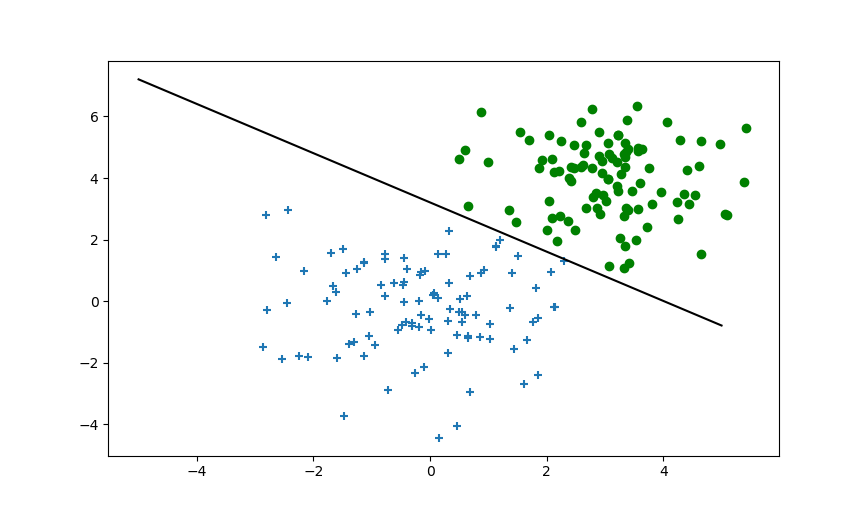
\includegraphics[scale=0.5]{Images/decisionboundaryIdeal.png}
    \\ ~~ \\
    This shows a clean boundary between the two classes.
\end{frame}

\begin{frame}{Decision Boundaries}
    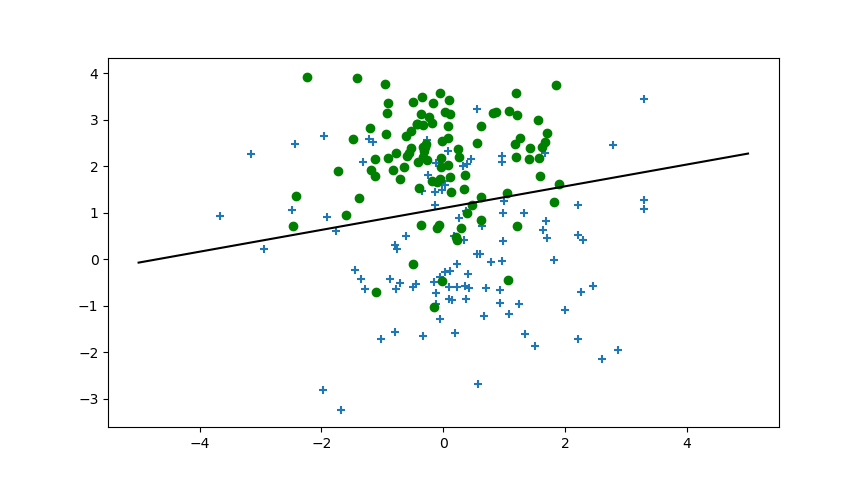
\includegraphics[scale=0.51]{Images/decisionboundaryRealistic.png}
    \\ ~~ \\
    This messy example is closer to reality.
\end{frame}

\begin{frame}{Conceptual Drift}
    The model we make today will represent the malware as a snapshot in time. Over time, malware changes, and new malware \& goodware samples will be needed, perhaps even new features as well, and today's model won't be as effective for future malware. What's the time frame? Probably weeks to months, maybe a year. It depends on a lot of variables.
\end{frame}

\begin{frame}
    Cyber data is hard! Most machine learning examples and models deal with data which is natively in two or three dimension, such as images. One dimensional data, such as malware or network traffic, is harder (but still do-able).
    \\ ~~ \\
    If your model is getting 100\% accuracy, what you really have is an error. We \textit{cannot} represent the entirety of the problem domain to the model, so it will always have some error.
\end{frame}

\begin{frame}[fragile]{False Positive Example}
\begin{columns}
    \column{0.5\textwidth}
\lstset{language=C,
    basicstyle=\tiny,
    keywordstyle=\color{blue}\ttfamily,
    stringstyle=\color{red}\ttfamily,
    commentstyle=\color{green}\ttfamily,
    morecomment=[l][\color{magenta}]{\#}
}
\begin{lstlisting}
#include<stdio.h>
#include<stdlib.h>

int main(int argc, char* argv[]) {
	printf("Test! Hello World!\n");
	return EXIT_SUCCESS;
}
\end{lstlisting}
\column{0.5\textwidth}
\begin{itemize}
    \item Mingw32: \href{https://www.virustotal.com/gui/file/0e0c92507aeaf6feec76cb8e3fa42bd4d1809e3d2987a6b6477155fd191c6cb1/detection}{22/67 hits}
    \item Mingw32 \& UPX: \href{https://www.virustotal.com/gui/file/25c6542b451a7279f833e3cf2e657f687cfcae68f48cd62afbe5a029bebe8294/detection}{17/69 hits}
    \item VS '19: \href{https://www.virustotal.com/gui/file/20ea89cad0c6ce3e1f38e50f8f3e5d37694fb3043862206db573516b47ac3611/detection}{2/71 hits}
    \item VS '19 \& UPX: \href{https://www.virustotal.com/gui/file/8ce853912e7b5f207aec7e2551925d16804e410432ed1ba1f99060b5562b8a62/detection}{8/70 hits}
\end{itemize}
\end{columns}
\\ ~~ \\ ~~ \\
The lesson? Don't rely on features that aren't correlated to the topic at hand.
\begin{itemize}
    \item File size
    \item Compiler identification
    \item Static builds
    \item High entropy
\end{itemize}
\end{frame}

\begin{frame}{False Positive Example VT}
    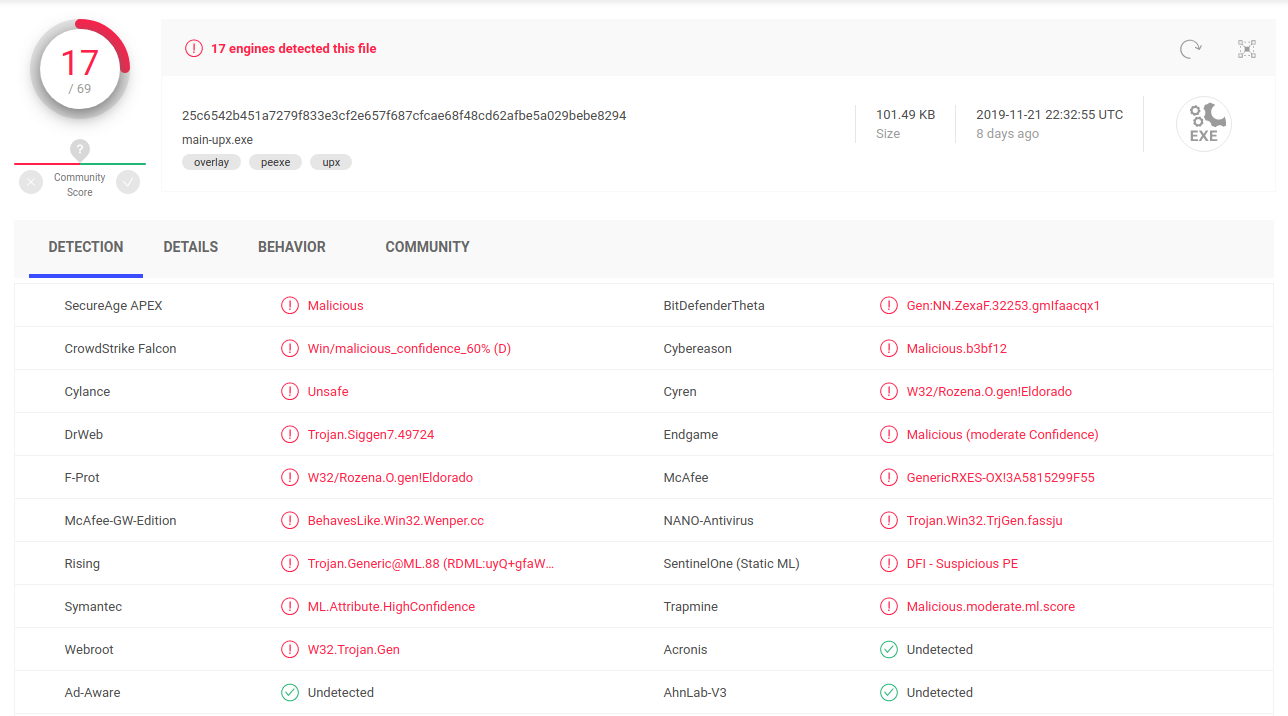
\includegraphics[scale=0.3]{Images/hello_world_mingw32_upx_VT.png}
\end{frame}

\begin{frame}[fragile]{False Positive Example 2}
    \lstset{language=Golang,
    basicstyle=\tiny,
    keywordstyle=\color{blue}\ttfamily,
    stringstyle=\color{red}\ttfamily,
    commentstyle=\color{green}\ttfamily,
    morecomment=[l][\color{magenta}]{\#}
}

\begin{columns}
    \column{0.5\textwidth}
\begin{lstlisting}
package main

import "fmt"

func main() {
    fmt.Println("Test! Hello World!")
}
\end{lstlisting}
\column{0.5\textwidth}
\begin{itemize}
    \item Original: \href{https://www.virustotal.com/gui/file/77ec22ff39c3fdbc4b6b567d6f56e66e271b02cb372b232247a9bf76340d9050/detection}{7/69 hits}
    \item Stripped: \href{https://www.virustotal.com/gui/file/6c4dba01b3e09dffd6172db0b5eff424a589f9a9010c6e6968ffb8019a440be7/detection}{4/69 hits}
    \item Stripped \& UPX: \href{https://www.virustotal.com/gui/file/833f164a685cc564b302c91e8bbca1c3f88291a0e566e52ac5b15c080e8aa21b/detection}{8/68 hits}
\end{itemize}

\end{columns}
\end{frame}

\begin{frame}{Lab 4}
    This week's Lab exercise is to identify characteristics of a file to use as features, create a model from the training data, and evaluate it's performance against the testing data. Change some of the features to measure the impact on accuracy.
    \\ ~~ \\
    A note about VMs: you may find that running code on the malware/goodware data in the VM is slow. Where needed, adjust your training and testing sizes so that the code runs in a reasonable amount of time, and document what these data sizes are. Allocating more CPU and RAM will improve performance, but this is dependant on your hardware.
    \\ ~~ \\
    For next week, please read \textit{Variant: A Malware Similarity Testing Framework} \attachfile{Papers/Variant_Malware_Testing_Framework.pdf}.
\end{frame}

\end{document}